%
% Chapter 4
%

\chapter{PHYSICS OBJECTS}
Each of the CMS subdetectors (neglecting the trigger system) technically only record and detect hits and energy deposits. While these hits and energy deposits are almost
always due to passing particles, the detectors themselves and more precisely the readouts, only produce information about the position, value, and multiplicity of
these hits and energy deposits. It is thanks to clever and accurate experimental techniques that we can reconstruct various particles from these hits and energy deposits.
In part because CMS does not detect particles directly, reconstructed particles are referred to as physics \emp{objects} in this context. Using
the term particles implies certainty about the identify of the object, and because there is some uncertainty, however small, inherent in the reconstruction, objects is
more accurate and widely used. The reconstruction technique varies greatly with different objects and the subdetectors used to detect and record their hits and energy
deposits. 

\section{Particle Flow}
The particle flow algorithm is used by CMS to reconstruct physics objects from hits and energy deposits. Particle Flow and CMS are unique in the sense
that nearly all physics analyses performed on data collected by CMS use objects reconstructed with this single algorithm. The primary advantage of this strategy is
uniform and consistent object definitions across nearly all papers published on behalf of CMS. Other collaborations such as ATLAS do not use
the same algorithm collaboration-wide. The purpose of particle flow is to identify all final-state stable particles in an event recorded by CMS, specifically electrons,
mouons, taus, jets and photons. Particle flow optimally combines building-block information (hits and energy clusters) from all subdetectors to reconstruct objects and
determine particle type, position, and momentum. It does this using 2 different primary reconstruction techniques for reconstructing tracks from tracker hits, and clusters
of energy deposits from individual calorimeter cells. 

\begin{figure}[hbtp]
 \begin{center}
   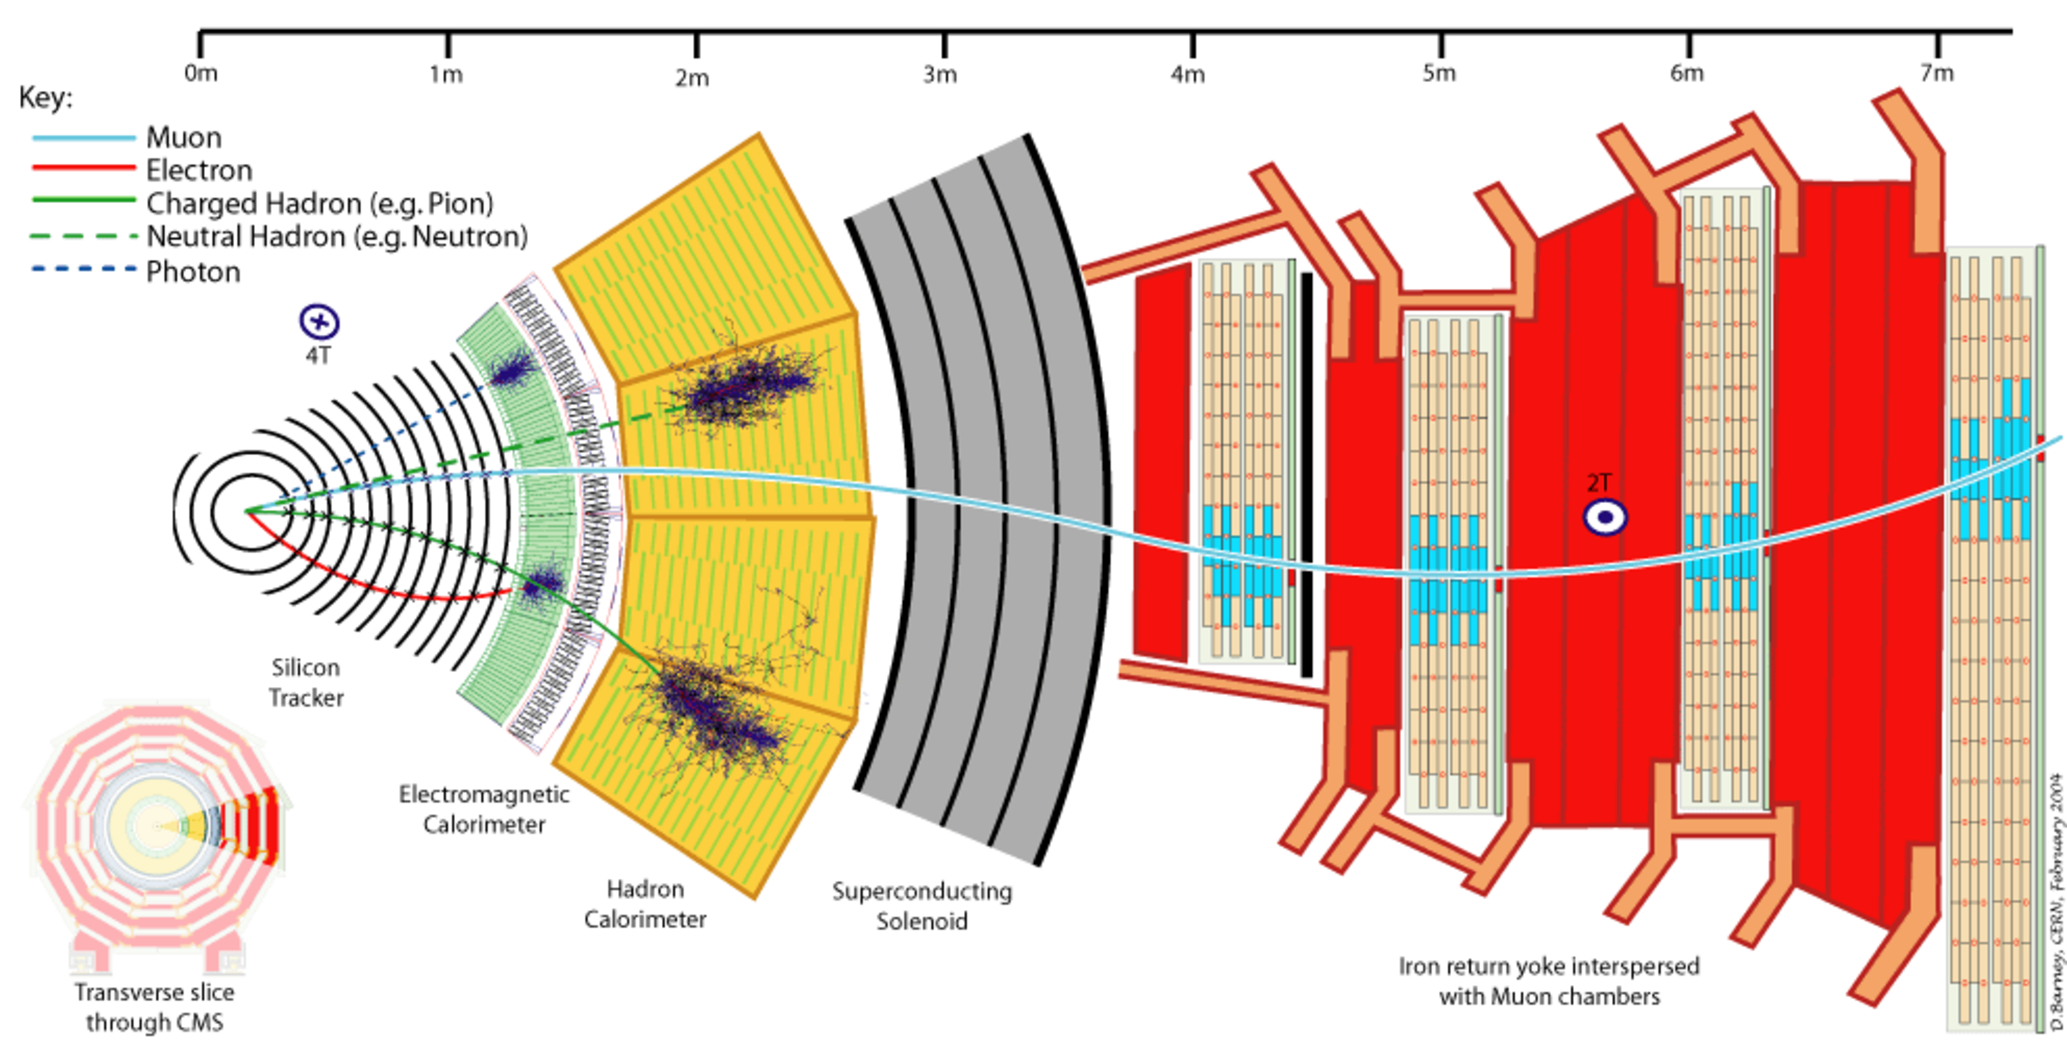
\includegraphics[width=0.8\textwidth]{ch4_figs/cms_particleflow.pdf}
   \caption{An overview of how CMS detects different types of particles. The slice of CMS in in the x-y plane.~\cite{NEED CITATION}.}
   \label{fig:cms_pflow}
 \end{center}
\end{figure}

Object reconstruction begins with grouping collections of hits into tracks in an iterative process~\cite{CMS-TRK-09-001}. In the first iteration, tracks are
seeded with initial hits and subject to very tight criteria, sacrificing efficiency for a low fake rate. In the following iterations, hits assigned to
tracks in the previous iteration are removed from further consideration, and the criteria for candidate tracks is gradually relaxed with each iteration. In the final iterations,
the constraints on the track seed are relaxed to account for secondary decays from photon conversions and nuclear interactions with the silicon tracker material. This technique
reconstructs tracks with as few as three hits and \pts as small as 150 MeV with a fake rate in the single digits~\cite{CMS-PFT-09-001}. A similar but separate track
reconstruction is performed in the muon chambers to reconstruct muon tracks. 

Object reconstruction continues in the calorimeters, where it relies on a clustering algorithm to identify individual energy deposits and associate them to an object. This
algorithm is designed to yield a high efficiency even for low energy, and nearby objects. The clustering process is performed separately in the ECAL and HCAL, and furthermore in
the barrel, and endcaps. The ECAL preshower also uses separate clusterings in each of its two layers. In the HF, no clustering is performed, where each module is considered an
independent cluster. The clustering algorithm begins by identifying cells (cluster seeds) with an energy above a given ``seed'' energy threshold. Clusters are then increased by
adding adjacent\footnote{sharing at least one edge with the seed} cells that have an energy above a given threshold. The calorimeter granularity is used to optimize the
determination of cluster energies and positions~\cite{CMS-PFT-09-001}.  

After the tracking and clustering is complete, Particle Flow then matches tracks in the tracker to energy clusters in the calorimeters, and to tracks in the muon chambers.
In a given event, there can be many different objects and Particle Flow utilizes
a process-of-elimination strategy. Because they are the easiest to identify unambiguously, muons are identified first by matching tracks in the inner tracker to the tracks in
the muon chambers. The matching criteria is based on a $\chi^{2}$ fit threshold. When multiple sets of tracks are matched, the set with the lowest $\chi^{2}$ is selected as the
muon object. Muons are first reconstructed this way and called global muons. Particle flow muons are identifed from global muons when the \pt~s measured in the tracker and the
muon chambers agree to within three standard deviations. The tracks corresponding to the muon object are then removed from consideration for the remaining object reconstruction. 

Following muons, electrons are reconstructed next. Because electrons deflect strongly in the magnetic field, they leave characteristically short tracks, and lose energy via
Bremsstrahlung radiation. The tracks are flagged based on these characteristics as potential electron candidates and refitted with a Gaussian-Sum Filter (GSF)~\cite{gsf} and the
resulting tracks are then matched to ECAL energy clusters. The Bremsstrahlung photons are emitted tangentially to electron track and this is accounted for in the ECAL clustering
and track matching specifically for electrons. These matches are then subject to additional quality criteria before they are considered particle flow electrons, and their
corresponding tracks and energy deposits removed from further consideration for the remaining object reconstruction. 

At this point in the event/object reconstruction, the so-called low lying fruit has been picked, and the more difficult objects are all that remain. These objects are charged
and neutral hadrons (jets), and photons. The neutral particles are difficult to reconstruct because they don't leave hits in the tracker, so only calorimeter information is
available. Photons are distinguished from neutral hadrons by separate ECAL and HCAL clusters. Photons interact with and are stopped by the ECAL, while the same is true for
neutral hadrons and the HCAL. Additional in-event calibration techniques are also used to further distinguish these objects. The remainig tracks are subject to tighter
quality cuts aimed at reducing the fake-rate. The high-quality tracks passing these thresholds are matched to ECAL and HCAL deposits, and give rise to particle flow 
charge hadrons. The momentum of these objects is measured from the track radius and compared to the corresponding energy deposit in the calorimeters assuming the object is
a charged pion. If the two measurements are compatible, the momenta is refined with additonal fits to the tracks and energy deposit(s)~\cite{CMS-PFT-09-001}. 





\section{Jets}
\section{Leptons}
\section{Taus}
\section{MET}

